% !TEX TS-program = pdflatex
% !TEX encoding = UTF-8 Unicode

% This is a simple template for a LaTeX document using the "article" class.
% See "book", "report", "letter" for other types of document.

\documentclass[11pt]{article} % use larger type; default would be 10pt

\usepackage[utf8]{inputenc} % set input encoding (not needed with XeLaTeX)

%%% Examples of Article customizations
% These packages are optional, depending whether you want the features they provide.
% See the LaTeX Companion or other references for full information.

%%% PAGE DIMENSIONS
\usepackage{geometry} % to change the page dimensions
\geometry{a4paper} % or letterpaper (US) or a5paper or....
% \geometry{margins=2in} % for example, change the margins to 2 inches all round
% \geometry{landscape} % set up the page for landscape
%   read geometry.pdf for detailed page layout information

\usepackage{graphicx} % support the \includegraphics command and options

% \usepackage[parfill]{parskip} % Activate to begin paragraphs with an empty line rather than an indent

%%% PACKAGES
\usepackage{booktabs} % for much better looking tables
\usepackage{array} % for better arrays (eg matrices) in maths
\usepackage{paralist} % very flexible & customisable lists (eg. enumerate/itemize, etc.)
\usepackage{verbatim} % adds environment for commenting out blocks of text & for better verbatim
\usepackage{subfig} % make it possible to include more than one captioned figure/table in a single float
% These packages are all incorporated in the memoir class to one degree or another...

%%% HEADERS & FOOTERS
\usepackage{fancyhdr} % This should be set AFTER setting up the page geometry
\pagestyle{fancy} % options: empty , plain , fancy
\renewcommand{\headrulewidth}{0pt} % customise the layout...
\lhead{}\chead{}\rhead{}
\lfoot{}\cfoot{\thepage}\rfoot{}

%%% SECTION TITLE APPEARANCE
\usepackage{sectsty}
\allsectionsfont{\sffamily\mdseries\upshape} % (See the fntguide.pdf for font help)
% (This matches ConTeXt defaults)

%%% ToC (table of contents) APPEARANCE
\usepackage[nottoc,notlof,notlot]{tocbibind} % Put the bibliography in the ToC
\usepackage[titles,subfigure]{tocloft} % Alter the style of the Table of Contents
\renewcommand{\cftsecfont}{\rmfamily\mdseries\upshape}
\renewcommand{\cftsecpagefont}{\rmfamily\mdseries\upshape} % No bold!

%%% END Article customizations

%%% The "real" document content comes below...

\title{CS577 FABL Project Report}
\author{Eric O'Connell and Matthaus Litteken}
\date{June 10, 2011}

\begin{document}
\maketitle

\section{LLVM backend for FAB}

\subsection{Resources \& Platforms}
We decided to build from the type-checked AST emitted by the reference implementation of FAB from CS322. We were interested in using an alternative to Java for the implementation of the compiler, and so wrote it using JRuby in order to have direct access to the AST object. We also decided that, rather than generate LLVM-IR as ascii text, we would use the API, which fortunately is available to JRuby through the Ruby FFI.

\subsection{Installation \& Running}
The source for the project can be found via our git repository (git@github.com:mlitteken/CS-577-Project.git).

\begin{itemize}
\item{Install LLVM 2.9: http://llvm.org/}
\item{Install JRuby: http://www.jruby.org/}
\item{Clone git repository: `git clone git@github.com:mlitteken/CS-577-Project.git`}
\item{using JRuby, `gem install ffi` and `gem install ruby-debug`}
\item{in the root of the source tree, jruby -J-classpath .:src:src/frontend.jar sandbox/integration.rb path/to/file.fab [none|half|full] [true|false]}
\end{itemize}

\subsection{The Design}

The compiler walks the AST, generating code for all top-level code and remembering functions to be generated later. We began our process by integrating the AST with JRuby. In order to do this, we had to modify Ast.java to add 'public' access qualifiers to all fields and methods, because although we were using Ruby's ability to re-open classes and add methods to them, the specific implementation which JRuby uses seems to insert a class shim, which rendered the package variables inaccessible to our code.

The actual walk of the AST was performed by functions which we added to the Java AST objects using the aformentioned open classes of Ruby. These ended up being quite similar, though slightly less indirect, than the visitor pattern methods we wrote in CS322. Each of these gen() methods took a context as a parmater, which handled some of the LLVM-related bookkeeping (such as setting the current function \& basic block) and maintaining a symbol table. The symbol table in the main branch simply resolved names to memory addresses (allocated by the LLVM alloca instruction), however in the unfinished 'closure' branch it was necessary to add "Resolvers" which mapped symbols to a tuple of (memory address, AST node) in order to preserve type information.

\subsection{Results}

LLVM optimizations are impressive, considering how easy it is to employ them. Most of them are simple to add, however the order in which they should be applied is not obvious or documented. By trial and error, and by noticing the large number of lines remaining in optimized code we added another mem2reg pass at the end of the optimizers. This reduced the total code size by almost 2/3 in some cases (see Figure 1). The assembly code lines include comments and other annotations, so comparing them may not be as exact as possible.

\begin{figure}[h!]
\caption{}
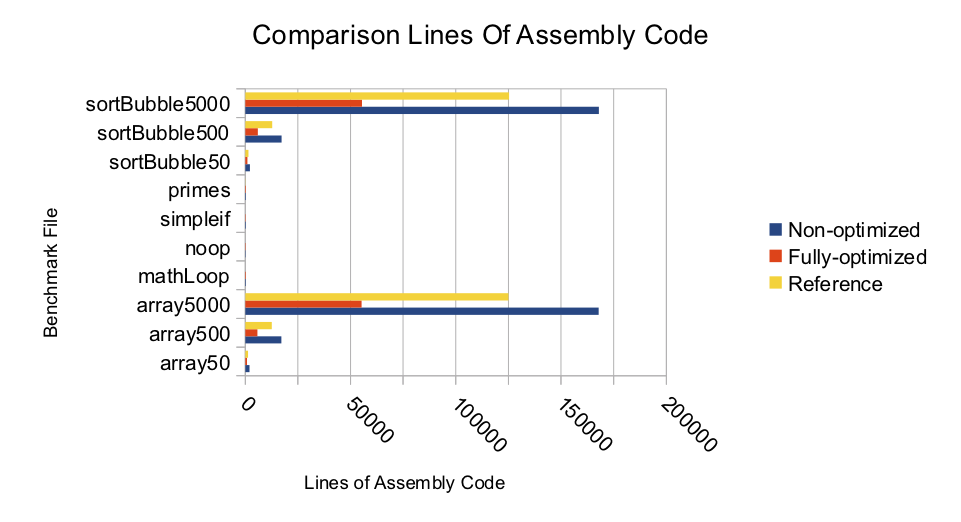
\includegraphics{sloc.png}
\end{figure}

In addition to reducing the number of lines of source assembly, the optimizer also greatly simplifies the CFG for the program at hand. As can be seen in Figures 2 and 3, the simpleif program is optimized from a CFG of six levels to a simple return of 0. In another case, constant variables from binary arithmetic operations were folded together to simplify a loop body (this was achieved using the instcombine optimization).

Even with the optimizations, the compiled binaries using the llvm toolchain were slower than the reference binary on the larger bubble sort set. Upon inspection, it appears as though the llvm based binary had more stack usage than the reference binary. These spills to memory no doubt slow the execution. The optimizer did improve the memory usage, but not to the level of the reference binary.

\begin{figure}[h!]
\caption{Unoptimized CFG for simpleif.fab}
\centering
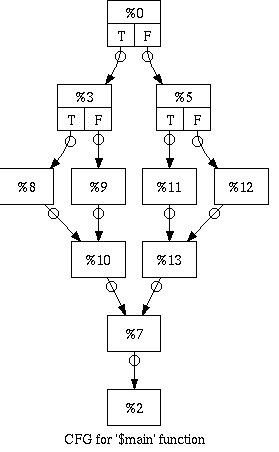
\includegraphics[width=50mm]{noOpt.png}
\caption{Fully optimized CFG for simpleif.fab}
\centering
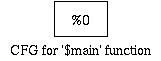
\includegraphics[width=25mm]{fullOpt.png}
\end{figure}

The most interesting benchmarks were the bubblesorts and array initializations of varying size, and the noop baseline. The noop baseline was informative, as it displays how much extra code is added to our implementation by default. 

We added the array initializations to see how much of the sort was building the array and how much was actual sorting. The compiled code took about the same amount of time to build the array in each of the sizes, while the interpreted code took an order of magnitude more for each additional order of magnitude of array elements.

Unsurprisingly, interpreting FAB was orders of magnitude slower than compiled FAB, especially with large arrays (see Tables 1 and 2). In general, the non-optimized llvm was interpreted far faster than the fully optimized or reference interpreters. This may have been because optimizations that were helpful for compilation weren't helpful for interpretation. The reference interpreter was normalized against the noop benchmark to eliminate as best as possible the parse and lex time in the benchmarks.

\begin{table}[h!]
\centering
\caption{Compiled Fab (on 500 iterations)}
\begin{tabular}{c | c | c | c }
Benchmark & Non-optimized & Fully Optimized & Reference\\ \hline
array50 & 12.827 & 11.719 & 12.238\\ \hline
array500 & 11.689 & 11.78 & 12.19\\ \hline
array5000 & 11.757 & 11.866 & 12.124\\ \hline
mathLoop & 11.616 & 11.776 & 12.171\\ \hline
noop & 11.735 & 11.808 & 12.174\\ \hline
simpleif & 11.876 & 12.319 & 11.923\\ \hline
primes (5 iterations) & 25.947 & 25.915 & 2.796\\ \hline
sortBubble50 & 12.414 & 12.025 & 11.781\\ \hline
sortBubble500 & 12.566 & 12.206 & 12.233\\ \hline
sortBubble5000 & 138.01 & 131.976 & 110.914\\ \hline
\end{tabular}
\end{table}

\begin{table}[h!]
\centering
\caption{Interpreted Fab (10 iterations normalized to 500 iterations)}
\begin{tabular}{c | c | c | c | c}
Benchmark & Non-optimized & Fully Optimized & Reference & Normalized Reference\\ \hline
array50 & 38.35 & 44.2 & 159.77 & 11.25\\ \hline
array500 & 273.00 & 880.35 & 171.67 & 23.15\\ \hline
array5000 & 6212.95 & 108014.8 & 260.96 & 112.44\\ \hline
mathLoop & 21.05 & 18.1 & 156.05 & 7.53\\ \hline
noop & 16.8 & 16.65 & 148.52 & 0\\ \hline
simpleif & 17.5 & 16.25 & 152.00 & 3.48\\ \hline
primes (5 iterations) & 26.032 & 25.983 & 113.642 & N/A\\ \hline
sortBubble50 & 42.2 & 41.04 & 176.47 & 27.95\\ \hline
sortBubble500 & 309.75 & 889.1 & 299.44 & 150.92\\ \hline
sortBubble5000 & 6663.95 & 139629.5 & 36867.5 & 36718.98\\ \hline
\end{tabular}
\end{table}

Some more other benchmarks were planned, but depended upon function and recursion support, which was not completed. Fibonacci as well as some currying were planned.

In general, the compiled llvm code was comparable to the reference compiler. It was a touch slower, but with the exception of the primes and 5000 element bubblesort, they were within a second in execution time over 500 iterations.


\subsection{Reflections}

After some initial hiccups in getting all of the components to talk to each other, the early development of FABL proceeded at a speedy pace. We began by simply re-writing the pretty-printer in JRuby by walking the AST and printing each node. The actual functionality was brought up starting from emitting integer constants, then simple arithmetic operations. In order to verify that arithmetic was working before any infrastructure was in place, a shim was inserted into the code generation which caused the value of the last VarDec node to be returned by the main function, which could then be printed out as a result of the JIT execution. 

The remaining functionality was built up generally from simple, straight-line code up towards more complex control structures. One particular challenge was in bringing up some of the runtime support like input, output, and memory allocation. Fortunately we were able to leverage on top of LLVM's linkage with libc, which allowed us to directly call printf, scanf, and malloc from within our generated code. We chose to wrap these directly in "hand-generated" LLVM functions which were then called from the code generators, for example in WriteSt. As a note, we did not implement any garbage collection (or error-checking for malloc!) so allocation will occur until available memory is consumed.

Adding closures to this implementation proved to be an extremely difficult challenge for a variety of reasons. One major problem seemed to be that the level of abstraction at which we were working was not high enough; mostly due to the decision to work directly from the AST. The AST is not linearized, in other words, function declarations are still nested, so not all functions are known at the time of code generation. As time was closing in on the deadline, we believe that a potential workaround to this would be to pre-generate all function pointers ahead of time (with empty function bodies) which could then be bound to the call sites in closure records. The compilation would proceed in this manner:

\begin{itemize}
\item{walk the entire AST without generating any code}
\item{as function declarations are encountered, create empty LLVM functions for them}
\item{bind these function pointers into the closure records as they are encountered during regular code generation}
\end{itemize}

We think this would be a suitable workaround which would enable us to avoid the full linearization process with just a simple pre-processing phase.

One other major challenge in this project has been ensuring that we generate the correct types; LLVM IR is fully typed, and in fact its API depends on having the correct types available during code generation: if an operation is performed on an instruction of the wrong type, in general the process will segfault. One particular instruction which proved unruly was getElementPointer. getElementPointer was often counterintuitive to use and difficult to debug. It would tend to either segfault or return a garbage/unitialized result.

LLVM's IR is strongly-typed. Constructing type signatures for a function which takes itself is "fun".. llvm-ruby's API is fairly well-adapted to Ruby idioms. However, as we were working on the project, some improvements have been made to the development branch would make some of the code nicer.

\subsection{Future Work}

We would like to complete the work to support full FAB function-calling semantics including closures and mutual-recursion. In addition, in order to test more of LLVM's optimization infrastructure, real numbers would open up the door to more numerical testing. LLVM includes primitives for assisting with garbage collection, although it does not provide a garbage collector.

Other items which could be given attention given more time would include some commenting of the code, for easier maintenance. Also, much of the llvm assembly we generate is overly verbose and inefficient. We could look at some of the changes that the initial optimizer passes make and see if any of that could be easily changed at the generation level of FABL.

One other task would be deciding the optimal order for the optimization passes. Some of them clearly depend upon or are aided by other passes, and we could find no stated optimal order in the llvm references. Figuring out which optimizations are most beneficial would also be a good thing to do and could enable us to reduce stack/memory usage and increase register usage, which would improve performance for our compiler.

A final instace of improvement would be to selectively include the print functions (write\_int, write\_bool, write\_string), instead of including them by default in every program.


\end{document}
